\chapter{Замкнутые струны, согласование уровней и дуальность}

\lectureoverview{Замкнутая струна допускает независимые волны в двух своих внутренних направлениях. При квантовании этих волн сначала кажется, что это просто удваивает фотон открытой струны, но инвариантность относительно сдвига начала струнной координаты устраняет односторонние состояния. Первый оставшийся уровень содержит безмассовую частицу со спином два. Та же идея смены описания затем ставит более широкий вопрос: когда константы связи изменяются, что вообще означает для какого-либо объекта быть фундаментальным?}

\section{Генератор, оставленный про запас}

Прежде чем рисовать замкнутую струну, восстановим один факт из канонической механики. Пусть
\begin{equation}
  L=L(q_i,\dot q_i),
\end{equation}
и определим импульс, сопряжённый с \(q_i\), как
\begin{equation}
  p_i=\frac{\partial L}{\partial\dot q_i}.
\end{equation}
Бесконечно малое непрерывное преобразование можно записать в виде
\begin{equation}
  \delta q_i=\epsilon f_i(q),
  \label{eq:l04-infinitesimal-transformation}
\end{equation}
где \(\epsilon\) — малый параметр. Если это преобразование является симметрией, теорема Нётер даёт сохраняющийся заряд. Разделив смещение координаты на общий параметр, получаем генератор
\begin{equation}
  Q=\sum_i p_i f_i(q)
   =\frac{1}{\epsilon}\sum_i p_i\,\delta q_i.
  \label{eq:l04-noether-charge}
\end{equation}
В квантовой механике \(Q\) — оператор, порождающий соответствующее малое преобразование.

Вращение в плоскости \(xy\) — привычный пример. При одном выборе ориентации
\begin{equation}
  \delta x=\epsilon y,
  \qquad
  \delta y=-\epsilon x,
\end{equation}
и \eqref{eq:l04-noether-charge} превращается в момент импульса с точностью до того же выбора знака. Сам по себе этот пример несуществен. Существенна схема: свёртка импульса с бесконечно малым смещением даёт генератор.

\begin{figure}[H]
  \centering
  \includegraphics[width=0.76\textwidth]{lecture_04_figure_01.png}
  \caption{Канонический импульс и нётеровский генератор, сохранённые для последующего сдвига координаты замкнутой струны.}
  \lectureframe{00:05:00}
  \label{fig:l04-noether-board}
\end{figure}

Вскоре мы встретим симметрию, координатой которой служит не точка в обычном пространстве, а нумерация точек вдоль струны. Уравнение \eqref{eq:l04-noether-charge} заранее держится под рукой именно для этой цели.

\section{Координата вдоль петли}

У замкнутой струны нет концов. Выберем параметр
\begin{equation}
  0\leq \sigma<2\pi
\end{equation}
и пока обозначим одну точку как \(\sigma=0\). Точка на полпути по обходу — это \(\sigma=\pi\); четверть оборота и три четверти оборота соответствуют \(\pi/2\) и
\(3\pi/2\). Эта отметка задаёт координатную договорённость, а не физическую особенность.

\begin{figure}[H]
  \centering
  \begin{minipage}[t]{0.58\textwidth}
    \centering
    \includegraphics[width=\textwidth]{lecture_04_figure_02.png}
    \par\smallskip\footnotesize (a) Отмеченная на доске петля.
  \end{minipage}\hfill
  \begin{minipage}[t]{0.37\textwidth}
    \centering
    \begin{adjustbox}{max width=\linewidth}
    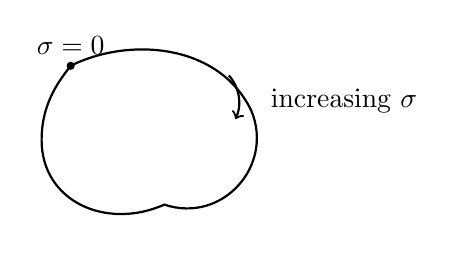
\begin{tikzpicture}[scale=0.82]
      \draw[thick]
        (0.1,1.1)
        .. controls (1.0,1.55) and (2.4,1.45) .. (2.9,0.4)
        .. controls (3.25,-0.45) and (2.45,-1.35) .. (1.55,-1.05)
        .. controls (0.65,-1.45) and (-0.35,-1.0) .. (-0.35,-0.05)
        .. controls (-0.35,0.55) and (-0.05,0.9) .. (0.1,1.1);
      \fill (0.1,1.1) circle (1.8pt);
      \node[above] at (0.1,1.12) {\(\sigma=0\)};
      \draw[->,thick] (2.55,0.95) arc[start angle=42,end angle=-25,radius=0.62];
      \node[right] at (3.05,0.55) {increasing \(\sigma\)};
    \end{tikzpicture}
    \end{adjustbox}
    \par\smallskip\footnotesize (b) Внутренняя ориентация.
  \end{minipage}
  \caption{Отмеченная точка задаёт начало отсчёта, а стрелка фиксирует направление, в котором возрастает
  \(\sigma\).}
  \lectureframe{00:06:48}
  \label{fig:l04-closed-string-origin}
\end{figure}

Стрелка вдоль петли задаёт \emph{внутреннюю} ориентацию. Её не следует путать с движением по часовой стрелке или против часовой стрелки в плоскости \(xy\). Представьте себе отмеченную резиновую ленту, которую подняли с доски, перевернули и положили обратно. Её видимое направление по часовой стрелке меняется на противоположное, тогда как последовательность её внутренних меток не меняется. Возрастание \(\sigma\) остаётся возрастанием \(\sigma\).

Это различие определяет язык право- и леводвижущихся волн. В этой главе праводвижущееся возмущение означает возмущение, распространяющееся в сторону возрастания \(\sigma\), а леводвижущееся — в сторону убывания \(\sigma\). Ни одно из этих названий не говорит, в какую сторону возмущение, по-видимому, движется в комнате.

Ориентация играла конкретную роль в исходной адронной картине струны. Разрыв ориентированной трубки потока даёт кварк на одном конце и антикварк на другом; внутренняя стрелка различает эти два конца. Можно строить и теории неориентированных струн, но в настоящем обсуждении мы сохраняем стрелку и оба направления вдоль неё.

\section{Периодичность и бегущие волны}

Пусть \(X(\sigma,\tau)\) и \(Y(\sigma,\tau)\) — две поперечные координаты струны, а \(\tau\) обозначает время. Дополнительные поперечные координаты, если они есть, рассматриваются в точности так же. Поскольку \(\sigma=0\) и
\(\sigma=2\pi\) обозначают одну и ту же точку,
\begin{equation}
  X(\sigma+2\pi,\tau)=X(\sigma,\tau),
  \qquad
  Y(\sigma+2\pi,\tau)=Y(\sigma,\tau).
  \label{eq:l04-periodicity}
\end{equation}

\begin{figure}[H]
  \centering
  \includegraphics[width=0.76\textwidth]{lecture_04_figure_03.png}
  \caption{Периодические граничные условия для двух поперечных координат.}
  \lectureframe{00:12:40}
  \label{fig:l04-periodicity-board}
\end{figure}

Следовательно, локализованное возмущение может циркулировать бесконечно долго. Когда оно достигает \(2\pi\), оно просто вновь появляется при \(0\). Это отличается от открытой струны, где бегущая волна доходит до конца и отражается; то, что было леводвижущимся, становится праводвижущимся, и наоборот. Стоячие волны естественны для открытой струны, тогда как замкнутая струна допускает два независимо распространяющихся семейства.

\subsection{Комплексные моды Фурье}

Удобным базисом для периодической функции служат
\begin{equation}
  e^{in\sigma}=\cos(n\sigma)+i\sin(n\sigma),
  \qquad n\in\mathbb Z.
\end{equation}
Требование целочисленности вынуждается периодичностью:
\(e^{in(\sigma+2\pi)}=e^{in\sigma}\). Замена \(n\), например, на полуцелое число изменила бы функцию после одного обхода.

Временно опуская зависимость от времени, получаем записанное на доске разложение
\begin{align}
  X(\sigma)
  &=
  X_0+
  \sum_{n>0}X_n e^{in\sigma}
  +\sum_{n>0}X_{-n}e^{-in\sigma},
  \label{eq:l04-fourier-x}\\
  Y(\sigma)
  &=
  Y_0+
  \sum_{n>0}Y_n e^{in\sigma}
  +\sum_{n>0}Y_{-n}e^{-in\sigma}.
  \label{eq:l04-fourier-y}
\end{align}
Для вещественных \(X\) и \(Y\) коэффициенты с отрицательными индексами на классическом уровне являются комплексно-сопряжёнными к коэффициентам с положительными индексами. Нулевые моды \(X_0\) и \(Y_0\) задают положение центра масс; это положения, а не внутренние колебания.

\begin{figure}[H]
  \centering
  \includegraphics[width=0.82\textwidth]{lecture_04_figure_04.png}
  \caption{Части периодического разложения Фурье с положительными и отрицательными индексами, за которыми следует нулевая мода.}
  \lectureframe{00:20:00}
  \label{fig:l04-fourier-board}
\end{figure}

\begin{classroomqa}
\audiencequestion{Если это бегущие волны, то где временная координата?\lecturetimestamp{00:19:05}}
\lecturerresponse{В записи на доске она лишь опущена. Бегущее решение несёт фазу, зависящую и от \(\sigma\), и от \(\tau\).
При соглашении, используемом ниже, одно семейство имеет
\(e^{-in(\tau-\sigma)}\), а другое —
\(e^{-in(\tau+\sigma)}\).}
\end{classroomqa}

Следовательно, распространение определяется полной фазой, а не само по себе знаком \(n\) в чисто пространственном Фурье-множителе. Можно написать
\begin{equation}
  X(\sigma,\tau)=X_R(\tau-\sigma)+X_L(\tau+\sigma),
  \label{eq:l04-chiral-solution}
\end{equation}
и аналогично для \(Y\). То, какое семейство обозначается как \(R\), а не \(L\), — вопрос соглашения; инвариантным фактом остаётся то, что вдоль окружности \(\sigma\) существуют два противоположных направления.\editorialnote{Множитель \(e^{in\sigma}\) в один фиксированный момент сам по себе не задаёт бегущую волну. Направление распространения определяется только после добавления временной фазы.}

\section{Энергия в двух направлениях}

Локальная динамика та же, что и у открытой струны. В используемой здесь упрощённой нормировке
\begin{equation}
  L\propto
  \int_0^{2\pi}d\sigma\,
  \left[
    \dot X^2-X'^2+\dot Y^2-Y'^2
  \right],
  \label{eq:l04-string-lagrangian}
\end{equation}
где точка обозначает \(\partial_\tau\), а штрих обозначает
\(\partial_\sigma\). В энергии между кинетическими и упругими членами стоит знак плюс:
\begin{equation}
  E\propto
  \int_0^{2\pi}d\sigma\,
  \left[
    \dot X^2+X'^2+\dot Y^2+Y'^2
  \right].
  \label{eq:l04-string-energy}
\end{equation}
Для любой поперечной координаты
\begin{equation}
  \dot X^2+X'^2
  =
  \frac12(\dot X+X')^2+
  \frac12(\dot X-X')^2.
  \label{eq:l04-energy-square-completion}
\end{equation}
Перекрёстные члены сокращаются, и остаются в точности исходные кинетическая и градиентная энергии.

\begin{figure}[H]
  \centering
  \includegraphics[width=0.82\textwidth]{lecture_04_figure_05.png}
  \caption{Полная энергия, перегруппированная по двум секторам бегущих волн.}
  \lectureframe{00:25:10}
  \label{fig:l04-energy-board}
\end{figure}

Для \(X_R(\tau-\sigma)\) имеем \(\dot X_R=-X_R'\); для
\(X_L(\tau+\sigma)\) имеем \(\dot X_L=X_L'\). Следовательно, два квадрата в \eqref{eq:l04-energy-square-completion} выделяют два хиральных
семейства. Учитывая все поперечные координаты, определим
\begin{align}
  E_L&\propto
  \frac12\int_0^{2\pi}d\sigma
  \sum_I(\dot X^I+X^{I\prime})^2,\\
  E_R&\propto
  \frac12\int_0^{2\pi}d\sigma
  \sum_I(\dot X^I-X^{I\prime})^2.
  \label{eq:l04-left-right-energies}
\end{align}
Тогда \(E=E_L+E_R\). Поскольку на этой стадии уравнения линейны, волны из двух секторов проходят друг сквозь друга без рассеяния.

\subsection{Вдвое больше осцилляторов}

Подстановка рядов Фурье в
\eqref{eq:l04-string-lagrangian} превращает каждый коэффициент ненулевой моды в гармонический осциллятор. Его частота пропорциональна \(|n|\): меньшая длина волны означает более высокую частоту и, следовательно, большую энергию возбуждения. В отличие от открытой струны, каждая положительная частота встречается в двух независимо распространяющихся копиях.

На доске операторы рождения с поляризацией по \(X\) обозначены как
\(a_n^+\) и \(a_{-n}^+\), а с поляризацией по \(Y\) — как
\(b_n^+\) и \(b_{-n}^+\). Чтобы яснее отделить создание от направления распространения, мы будем писать
\begin{equation}
  a_n^\dagger,\quad b_n^\dagger,
  \qquad
  \widetilde a_n^\dagger,\quad\widetilde b_n^\dagger,
  \qquad n>0.
  \label{eq:l04-oscillator-notation}
\end{equation}
Операторы без тильды и с тильдой создают противоположные направления на мировом листе; \(a\) и \(b\) обозначают две поперечные поляризации.

\begin{figure}[H]
  \centering
  \includegraphics[width=0.65\textwidth]{lecture_04_figure_06.png}
  \caption{Обозначения на доске для удвоенного набора операторов рождения с \(X\)- и \(Y\)-поляризацией.}
  \lectureframe{00:29:10}
  \label{fig:l04-oscillators-board}
\end{figure}

Если \(N_n^{(a)},N_n^{(b)}\) и их тильдованные аналоги — это числа заполнения, то осцилляторные уровни в двух направлениях схематически имеют вид
\begin{equation}
  \begin{aligned}
    N&=\sum_{n>0}n\bigl(N_n^{(a)}+N_n^{(b)}+\cdots\bigr),\\
    \widetilde N&=\sum_{n>0}n
      \bigl(\widetilde N_n^{(a)}+\widetilde N_n^{(b)}+\cdots\bigr).
  \end{aligned}
  \label{eq:l04-level-operators}
\end{equation}
Многоточия обозначают дополнительные поперечные направления.

\section{Неудачное предположение о спектре}

Напомним первый уровень открытой струны. Действие \(a_1^\dagger\) или \(b_1^\dagger\) на основное состояние даёт две линейные поляризации. Их круговые комбинации,
\begin{equation}
  c_\pm^\dagger
  =
  \frac{1}{\sqrt2}
  \left(a_1^\dagger\pm i b_1^\dagger\right),
  \label{eq:l04-open-circular}
\end{equation}
несут спиральность \(h=\pm1\). Отсутствие партнёра со спиральностью нуль является признаком безмассового вектора в этом элементарном четырёхмерном описании.

Пусть основное состояние замкнутой струны имеет квадрат массы \(m_0^2\). Первая, наивная догадка состоит в том, чтобы один раз подействовать любым из операторов
\begin{equation}
  a_1^\dagger,\quad b_1^\dagger,\quad
  \widetilde a_1^\dagger,\quad\widetilde b_1^\dagger.
  \label{eq:l04-naive-one-sided}
\end{equation}
Это похоже на две копии фотона открытой струны, по одной для каждого направления распространения. Однако на следующем энергетическом уровне неограниченный список не складывается в разумные вращательные мультиплеты. Более изощрённый учёт этого не исправляет. Предпосылка, что любой осцилляторный моном является физическим состоянием, неверна.

\subsection{Согласование уровней: сначала как правило}

Физическое условие для замкнутой струны имеет вид
\begin{equation}
  N=\widetilde N,
  \qquad\text{equivalently}\qquad E_L=E_R.
  \label{eq:l04-level-matching}
\end{equation}
Пока примем это как постулат; его происхождение будет выведено лишь после того, как мы увидим, чего оно позволяет добиться.

Каждое состояние в \eqref{eq:l04-naive-one-sided} имеет одну единицу энергии в одном секторе и ни одной в другом, так что исключаются они все. Первые сохраняющиеся состояния содержат по одному осциллятору из каждого семейства:
\begin{align}
  a_1^\dagger\widetilde a_1^\dagger\ket{0},
  &\qquad
  b_1^\dagger\widetilde b_1^\dagger\ket{0},
  \label{eq:l04-four-matched-a}\\
  a_1^\dagger\widetilde b_1^\dagger\ket{0},
  &\qquad
  b_1^\dagger\widetilde a_1^\dagger\ket{0}.
  \label{eq:l04-four-matched-b}
\end{align}
Их полная осцилляторная энергия равна 2 и поровну разделена между двумя направлениями. Один оператор рождения \(n=2\) имеет ту же полную осцилляторную энергию, но не удовлетворяет \eqref{eq:l04-level-matching}; он вносит две единицы только в один сектор.

\begin{figure}[H]
  \centering
  \includegraphics[width=0.70\textwidth]{lecture_04_figure_07.png}
  \caption{Четыре состояния первого уровня, которые проходят условие согласования уровней. На доске используются нижние индексы \(1\) и \(-1\) там, где в \eqref{eq:l04-four-matched-a}--\eqref{eq:l04-four-matched-b} используются операторы без тильды и с тильдой.}
  \lectureframe{00:41:05}
  \label{fig:l04-level-matched-board}
\end{figure}

\section{Гравитон на первом согласованном уровне}

Перейдём для обоих хиральных семейств к циркулярному базису:
\begin{equation}
  c_\pm^\dagger
  =\frac{a_1^\dagger\pm i b_1^\dagger}{\sqrt2},
  \qquad
  \widetilde c_\pm^\dagger
  =\frac{\widetilde a_1^\dagger\pm i\widetilde b_1^\dagger}{\sqrt2}.
  \label{eq:l04-closed-circular}
\end{equation}
Каждый множитель вносит спиральность \(+1\) или \(-1\) в обычном поперечном пространстве. Поэтому их произведения дают
\begin{center}
\begin{tabular}{c c}
  \toprule
  Состояние & Спиральность \\
  \midrule
  \(c_+^\dagger\widetilde c_+^\dagger\ket0\) & \(+2\) \\
  \(c_-^\dagger\widetilde c_-^\dagger\ket0\) & \(-2\) \\
  \(c_+^\dagger\widetilde c_-^\dagger\ket0\) & \(0\) \\
  \(c_-^\dagger\widetilde c_+^\dagger\ket0\) & \(0\) \\
  \bottomrule
\end{tabular}
\end{center}

\begin{classroomqa}
\audiencequestion{Должен ли второй множитель циркулярной поляризации происходить из противоположного сектора распространения?\lecturetimestamp{00:43:20}}
\lecturerresponse{Да. Первое выражение, написанное на доске, было исправлено именно по этой причине. Физическое состояние здесь должно сочетать один праводвижущийся осциллятор с одним леводвижущимся; иначе оно не согласовано по уровню. Спиральности относятся к поляризации в поперечном пространстве, тогда как два множителя относятся к противоположным направлениям на мировом листе.}
\end{classroomqa}

\begin{figure}[H]
  \centering
  \includegraphics[width=0.82\textwidth]{lecture_04_figure_08.png}
  \caption{Четыре произведения в циркулярном базисе после исправления на доске, со спиральностями \(+2,-2,0,0\).}
  \lectureframe{00:46:10}
  \label{fig:l04-helicity-board}
\end{figure}

Массивная частица со спином 2 имеет пять проекций спина,
\begin{equation}
  m=2,1,0,-1,-2.
\end{equation}
На согласованном уровне нет состояний-партнёров \(m=\pm1\). Поэтому он не может быть мультиплетом массивной частицы со спином 2. Напротив, безмассовая частица со спином 2 имеет только спиральности \(+2\) и \(-2\). Произведения с одинаковой спиральностью — это в точности эти два состояния: они и являются поляризациями гравитона.

Остаются две комбинации со спиральностью нуль. В терминологии, использованной на лекции, одна из них — дилатон, а другая — аксион. Ковариантное описание общего случая замкнутой бозонной струны уточняет это утверждение:
\begin{equation}
  \begin{aligned}
    \alpha_{-1}^{I}\widetilde\alpha_{-1}^{J}\ket{0;k}
    &\longrightarrow
    \underbrace{h_{IJ}}_{\text{symmetric traceless}}
    \oplus
    \underbrace{B_{IJ}}_{\text{antisymmetric}}\\
    &\hspace{2.5em}\oplus
    \underbrace{\Phi}_{\text{trace}}.
  \end{aligned}
  \label{eq:l04-massless-tensor-decomposition}
\end{equation}
Это гравитон, антисимметричная 2-форма и дилатон. В четырёх измерениях 2-форму можно дуализовать в аксионоподобный псевдоскаляр; именно такой язык использовался на лекции.\editorialnote{Второе состояние со спиральностью нуль в общем спектре замкнутой струны по существу является антисимметричным тензорным полем
\(B_{\mu\nu}\). Называть его аксионом — значит использовать четырёхмерное дуальное описание.}

На этом формальном уровне все три поля безмассовы. Компактификация, проекции и динамика фона могут изменить, какие скалярные или двухформенные степени свободы остаются лёгкими. С гравитоном дело обстоит иначе: как только имеется согласованный взаимодействующий сектор замкнутых струн, его безмассовое состояние со спином 2 неизбежно. Поэтому гравитация возникает из замкнутых струн, а не добавляется как отдельный ингредиент.

\section{Почему уровни должны согласовываться}

Теперь вернёмся к метке при \(\sigma=0\). Является ли она физической бусиной, прикреплённой к петле, или всего лишь началом отсчёта нашего параметра? Для обычной немаркированной замкнутой струны никакая точка не должна быть выделенной. Квантовое состояние должно оставаться неизменным, когда все метки сдвигаются одновременно.

\subsection{Дискретная версия}

Регуляризуем петлю как \(M\) упорядоченных точек с поперечными координатами \((X_i,Y_i)\). Временно опустим \(Y_i\). Волновая функция в конфигурационном пространстве имеет вид
\begin{equation}
  \Psi(X_1,X_2,\ldots,X_M).
\end{equation}
Изменение того, какая точка считается первой, даёт циклическую перестановку:
\begin{align}
  \Psi(X_1,X_2,\ldots,X_M)
  &=
  \Psi(X_2,\ldots,X_M,X_1)\nonumber\\
  &=
  \Psi(X_3,\ldots,X_M,X_1,X_2).
  \label{eq:l04-cyclic-wavefunction}
\end{align}
Это не инвариантность относительно произвольной перестановки. Например, если вставить \(X_3\) между \(X_1\) и \(X_2\), то изменится структура соседства и фактически произойдёт разрыв и повторное соединение дискретизованной струны. Только общее циклическое перенумерование
\begin{equation}
  X_i\longrightarrow X_{i+1}\qquad(\text{mod }M)
  \label{eq:l04-discrete-shift}
\end{equation}
выражает отсутствие выделенного начала отсчёта.

\begin{figure}[H]
  \centering
  \includegraphics[width=0.82\textwidth]{lecture_04_figure_09.png}
  \caption{Циклические тождества для волновой функции дискретизованной замкнутой струны.}
  \lectureframe{00:56:20}
  \label{fig:l04-cyclic-board}
\end{figure}

\subsection{Континуальная версия}

В континуальном пределе \(M\to\infty\) состояние задаётся волновым функционалом
\begin{equation*}
  \Psi[X(\sigma),Y(\sigma)].
\end{equation*}
Циклическое переобозначение превращается в
\begin{equation}
  \sigma\longrightarrow\sigma+\epsilon.
\end{equation}
Инвариантность означает
\begin{equation}
  \Psi[X(\sigma+\epsilon),Y(\sigma+\epsilon)]
  =
  \Psi[X(\sigma),Y(\sigma)].
  \label{eq:l04-wavefunctional-invariance}
\end{equation}

\begin{figure}[H]
  \centering
  \includegraphics[width=0.72\textwidth]{lecture_04_figure_10.png}
  \caption{Дискретный сдвиг и его континуальная форма для волнового функционала.}
  \lectureframe{00:58:40}
  \label{fig:l04-wavefunctional-board}
\end{figure}

В первом порядке,
\begin{equation}
  \delta X(\sigma)=\epsilon X'(\sigma),
  \qquad
  \delta Y(\sigma)=\epsilon Y'(\sigma),
  \label{eq:l04-profile-shift}
\end{equation}
с точностью до общего знака, который отличает активный сдвиг профиля от пассивного сдвига координаты. Соответствующее изменение волнового функционала равно
\begin{equation}
  \delta\Psi
  =
  \epsilon\int_0^{2\pi}d\sigma
  \left[
    \frac{\delta\Psi}{\delta X(\sigma)}X'(\sigma)
    +
    \frac{\delta\Psi}{\delta Y(\sigma)}Y'(\sigma)
  \right].
  \label{eq:l04-functional-variation}
\end{equation}

\begin{figure}[H]
  \centering
  \includegraphics[width=0.72\textwidth]{lecture_04_figure_11.png}
  \caption{Разложение сдвинутого аргумента волнового функционала по первому порядку.}
  \lectureframe{01:01:31}
  \label{fig:l04-functional-expansion-board}
\end{figure}

\begin{classroomqa}
\audiencequestion{Является ли условие первого порядка отдельным уравнением для каждого значения \(\sigma\)?\lecturetimestamp{01:01:30}}
\lecturerresponse{Нет. Преобразование сдвигает вместе каждую точку струны. Изменение в одной точке нужно сложить с изменениями во всех остальных, поэтому в континуальном выражении и появляется интеграл по \(\sigma\).}
\end{classroomqa}

В координатном представлении,
\begin{equation}
  P_X(\sigma)=-i\frac{\delta}{\delta X(\sigma)},
  \qquad
  P_Y(\sigma)=-i\frac{\delta}{\delta Y(\sigma)}
  \label{eq:l04-functional-momenta}
\end{equation}
при \(\hbar=1\). Поэтому уравнение \eqref{eq:l04-functional-variation} порождается оператором
\begin{equation}
  G_\sigma=
  \int_0^{2\pi}d\sigma\,
  \left[
    P_X(\sigma)X'(\sigma)+P_Y(\sigma)Y'(\sigma)
  \right].
  \label{eq:l04-sigma-generator}
\end{equation}
Это в точности нётеровская схема \eqref{eq:l04-noether-charge}: канонический импульс, умноженный на смещение координаты, с суммированием по всем степеням свободы. Состояние немаркированной замкнутой струны удовлетворяет
\begin{equation}
  G_\sigma\ket{\mathrm{phys}}=0.
  \label{eq:l04-physical-generator-condition}
\end{equation}

Для нормировки, принятой в \eqref{eq:l04-string-lagrangian},
\(P_I\propto\dot X^I\), так что то же условие записывается как
\begin{equation}
  \int_0^{2\pi}d\sigma
  \sum_I\dot X^I X^{I\prime}=0.
  \label{eq:l04-momentum-constraint}
\end{equation}

\begin{figure}[H]
  \centering
  \includegraphics[width=0.75\textwidth]{lecture_04_figure_12.png}
  \caption{Интегральный генератор после отождествления производной волнового функционала с импульсом.}
  \lectureframe{01:05:10}
  \label{fig:l04-generator-board}
\end{figure}

\subsection{Генератор — это разность энергий}

Сумма двух выражений в \eqref{eq:l04-left-right-energies} есть полная энергия. Их разность равна
\begin{align}
  E_L-E_R
  &\propto
  \frac12\int_0^{2\pi}d\sigma\sum_I
  \left[
    (\dot X^I+X^{I\prime})^2\right.\nonumber\\[-0.25em]
  &\hspace{7em}\left.
    -(\dot X^I-X^{I\prime})^2
  \right]\\
  &=
  2\int_0^{2\pi}d\sigma\sum_I
  \dot X^I X^{I\prime}.
  \label{eq:l04-energy-difference}
\end{align}
Этот интеграл и есть генератор, который должен аннигилировать физическое состояние. Следовательно,
\begin{equation}
  E_L-E_R=0,
  \qquad\text{or}\qquad
  N-\widetilde N=0.
\end{equation}
Согласование уровней утверждает, что начало отсчёта координаты \(\sigma\) ненаблюдаемо.

\begin{figure}[H]
  \centering
  \includegraphics[width=0.78\textwidth]{lecture_04_figure_13.png}
  \caption{Сумма и разность энергий, выписанные вместе в конце вывода условия согласования уровней.}
  \lectureframe{01:06:40}
  \label{fig:l04-energy-difference-board}
\end{figure}

\begin{classroomqa}
\audiencequestion{Почему в выписанных формулах множитель одна вторая, по-видимому, стоит по-разному?\lecturetimestamp{01:06:28}}
\lecturerresponse{Используется лишь относительная структура. Если восстановить одну согласованную общую нормировку, множитель одна вторая появляется в тождестве с выделением полного квадрата \eqref{eq:l04-energy-square-completion}. Сумма даёт полную энергию, тогда как разность остаётся пропорциональной \(\int d\sigma\,\dot X X'\). Обращение этой величины в нуль, а значит и согласование уровней, не зависит от этого общего соглашения.}
\end{classroomqa}

Это ограничение отбрасывает значительную часть наивного осцилляторного спектра и именно те состояния, из которых не получались разумные мультиплеты частиц. Оно не отбрасывает фотон открытой струны, потому что у открытой струны нет двух независимых циркулирующих секторов, подчинённых этому условию для замкнутой петли. Для замкнутой струны оно оставляет гравитон, дилатон, антисимметричное тензорное или аксионоподобное состояние и более высокие согласованные уровни.
\editorialnote{В ковариантном квантовании струны согласование уровней есть условие на нулевую моду \(L_0-\widetilde L_0=0\), одно из условий системы ограничений мирового листа. Приведённый здесь вывод выделяет его интуитивное происхождение как инвариантность относительно трансляций вдоль замкнутой струны.}

\section{Два смысла слов левый и правый}

Теперь есть два не связанных друг с другом употребления терминов «левый» и «правый»:
\begin{enumerate}
  \item \(X_R(\tau-\sigma)\) и \(X_L(\tau+\sigma)\) обозначают распространение
  в противоположных направлениях вдоль собственного круга \(\sigma\).
  \item \(c_+^\dagger\) и \(c_-^\dagger\) обозначают круговую поляризацию в
  физической поперечной плоскости \(xy\).
\end{enumerate}
В согласованном по уровням состоянии гравитона имеется по одному осциллятору из каждого направления мирового листа. Тем не менее эти два осциллятора могут иметь одинаковую геликальность в пространстве-времени, давая \(h=+2\) или \(h=-2\). Если смешать эти два смысла левого и правого, спектр будет казаться противоречивым, хотя на самом деле это не так.

\section{Что значит «фундаментальный»?}

После того как открытые и замкнутые струны квантованы на этом элементарном уровне, остаётся естественный вопрос: являются ли струны окончательными составляющими или они сами могут быть сделаны из чего-то ещё?

\begin{classroomqa}
\audiencequestion{Есть ли свидетельства или основания считать струны наиболее фундаментальными объектами, под которыми уже нет ничего меньшего?\lecturetimestamp{01:10:44}}
\lecturerresponse{Полезного ответа, не зависящего от параметров, нет. Степени свободы, которые в одном режиме выглядят элементарными, в другом могут стать тяжёлыми, протяжёнными и по-видимому составными. «Фундаментальный» лучше всего понимать как утверждение о том, какие переменные дают полезное описание при рассматриваемом значении связи.}
\end{classroomqa}

Электрические и магнитные заряды дают наиболее ясную модель такого ответа. Предположим, что теория содержит электрический заряд \(e\) и магнитный заряд \(g\). Ненаблюдаемая нить Дирака, прикреплённая к монополю, требует
\begin{equation}
  eg=2\pi n,
  \qquad n\in\mathbb Z.
  \label{eq:l04-dirac-quantization}
\end{equation}
Для минимальных зарядов \(n=1\). Тогда заряженная частица, обходящая нить Дирака, получает фазовый множитель \(e^{ieg}=1\), так что вспомогательную нить нельзя обнаружить.

\begin{figure}[H]
  \centering
  \begin{minipage}[t]{0.58\textwidth}
    \centering
    \includegraphics[width=\textwidth]{lecture_04_figure_14.png}
    \par\smallskip\footnotesize (a) Квантование Дирака на доске.
  \end{minipage}\hfill
  \begin{minipage}[t]{0.36\textwidth}
    \centering
    \begin{adjustbox}{max width=\linewidth}
    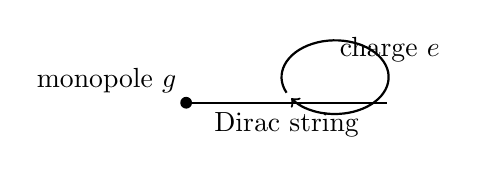
\begin{tikzpicture}[scale=0.85]
      \fill (0,0) circle (2.5pt);
      \node[above left] at (0,0) {monopole \(g\)};
      \draw[thick] (0,0) -- (3.0,0);
      \node[below] at (1.5,0) {Dirac string};
      \draw[->,thick] (1.5,0.15) arc[start angle=205,end angle=-145,
        x radius=0.8,y radius=0.55];
      \node[right] at (2.15,0.8) {charge \(e\)};
    \end{tikzpicture}
    \end{adjustbox}
    \par\smallskip\footnotesize (b) Фазовый эксперимент вокруг нити.
  \end{minipage}
  \caption{Согласно условию Дирака, электрический и магнитный заряды обратно пропорциональны.}
  \lectureframe{01:13:20}
  \label{fig:l04-dirac-board}
\end{figure}

Если \(e\) мало, обычная теория возмущений в электрических переменных полезна. Диаграммы Фейнмана с дополнительными электрическими вершинами подавляются всё сильнее. Но из \eqref{eq:l04-dirac-quantization} тогда следует, что \(g\) становится большим, так что диаграмматическое разложение по магнитным вершинам непригодно. В терминах обычных безразмерных констант связи,
\begin{equation}
  \alpha_e=\frac{e^2}{4\pi},
  \qquad
  \alpha_m=\frac{g^2}{4\pi},
  \qquad
  \alpha_e\alpha_m=\frac{n^2}{4}.
  \label{eq:l04-dual-couplings}
\end{equation}
Слабая электрическая связь соответствует сильной магнитной, и наоборот.

Монополь при сильной связи выглядит сложным и с точки зрения электрического описания. Его энергия поля велика; он одет интенсивным облаком флуктуаций калибровочного поля и виртуальных магнитно заряженных пар. Он ведёт себя как тяжёлый протяжённый объект и потому служит плохой отправной точкой для электрического ряда возмущений. Это не доказывает, что он менее фундаментален. Это говорит о том, что для этого режима он является неподходящей элементарной переменной.

Теперь представьте, что \(e\) непрерывно увеличивается. Условие квантования заставляет \(g\) уменьшаться. Вблизи самодуальной области ни одно описание не является особенно слабосвязанным, а по ту сторону неё магнитные переменные могут стать более простыми и лёгкими, тогда как электрические объекты становятся сильно одетыми. То, какой заряд следует называть элементарным, изменилось, хотя физическое содержание теории не изменилось.

\subsection{Вопрос Вигнера}

Эта неоднозначность однажды всплыла в обсуждении того, является ли бозон Хиггса фундаментальным или составным. Юджин Вигнер снова и снова спрашивал, что значит «составной». Один из предложенных критериев был связан с распадом: возможно, фундаментальный объект распадаться не может, а составной может. Но атом водорода в основном состоянии распадаться не может и при этом явно составной; протон может быть стабильным, тогда как нейтрон распадается, однако это не делает один из них элементарным, а другой составным в подразумеваемом смысле. Каждое простое определение порождало новый контрпример.

Герардус 'т Хоофт завершил обсуждение операциональным критерием: объект фундаментален тогда, когда его полезно считать фундаментальным. Это не уклонение. В нём признаётся, что «элементарный» выделяет переменные, в которых динамика проста, а простота может зависеть от константы связи и среды.

\section{К М-теории}

Теория струн реализует этот обмен ролями особенно резко. В одном режиме параметров струны лёгки и пертурбативны, тогда как D-браны выглядят как тяжёлые солитонные составные объекты, построенные из струнных степеней свободы. По мере изменения параметров D-браны могут стать более лёгкими элементарными объектами, а конфигурации, описываемые в первом режиме как струны, могут быть переинтерпретированы в их терминах. То, что выглядело фундаментальным, может стать составным; то, что выглядело составным, может стать фундаментальным.

Старая редукционистская картина предполагает однонаправленный спуск от больших объектов к меньшим составляющим и в конце концов к единственному нижнему слою. Дуальность подсказывает нечто менее линейное: по мере изменения констант связи описания могут переходить друг в друга, и не существует единственного набора переменных, выделенного повсюду. Именно с этой точки зрения будет рассматриваться следующая тема — М-теория.

Вопросы о том, почему критическая размерность для бозонной струны равна 26, а для суперструны — 10, здесь остаются открытыми. Вместо того чтобы, прежде чем двигаться дальше, разрешить каждый технический вопрос, мы теперь меняем точку зрения и спрашиваем, как М-теория может порождать теорию струн в подходящем пределе.